\documentclass{cernatsnote}
\usepackage{physics}
\usepackage{tcolorbox}
\tcbuselibrary{skins}
\usepackage{lipsum}
\usepackage{mathtools}
\usepackage{amsfonts}
\usepackage[colorinlistoftodos]{todonotes}
\usepackage{placeins}
\usepackage{amsmath}
\usepackage{physics}
\usepackage{tcolorbox}
\tcbuselibrary{skins}
\usepackage{lipsum}
\usepackage{amsmath}
\usepackage[T1]{fontenc}
\usepackage{graphicx, subfigure}
\usepackage{fancyhdr}
\usepackage{lmodern}
\usepackage{color}
\usepackage{transparent}
\usepackage{amsfonts}
\usepackage{mathtools}
\usepackage{tikz}
\usetikzlibrary{positioning}
\usepackage{pgfplots}
\pgfplotsset{compat=1.10}
\usepackage{textcomp}
\usepackage{float}
\usepackage{adjustbox} % Used to constrain images to a maximum size 
\usepackage{color} % Allow colors to be defined
\usepackage{enumerate} % Needed for markdown enumerations to work
\usepackage{geometry} % Used to adjust the document margins
\usepackage{amsmath} % Equations
\usepackage{amssymb}
\usepackage{fancyvrb} % verbatim replacement that allows latex
\usepackage{grffile} % extends the file name processing of package graphics 
                         % to support a larger range 
    % The hyperref package gives us a pdf with properly built
    % internal navigation ('pdf bookmarks' for the table of contents,
    % internal cross-reference links, web links for URLs, etc.)
\usepackage{hyperref}
\usepackage{longtable} % longtable support required by pandoc >1.10
\usepackage{tabularx}
\usepackage{epigraph}
\usepackage{quotchap}
\usepackage{lscape}
\usepackage{enumerate}
\usepackage{xpatch}
\usepackage{titletoc}
\usepackage{float}	
\usepackage{xparse}
\NewDocumentCommand{\DIV}{om}{%
  \IfValueT{#1}{\setcounter{#2}{\numexpr#1-1\relax}}%
  \csname #2\endcsname
}

\newtcolorbox{mybox}[3][]
{
  colframe = #2!25,
  colback  = #2!10,
  coltitle = #2!20!black,  
  title    = {#3},
  #1,
}

%\renewcommand{\thesubsection}{\thesection.\alph{subsection}}


\title{Computational Physics – Exercise 6}
\author{Pugazharasu Anancia Devaneyan, Rishi Kumar Senthil Kumar}
\email{\href{pugs@uni-bonn.de}{pugs@uni-bonn.de}, \href{s6risent@uni-bonn.de}{s6risent@uni-bonn.de}}
\date{\today}

\begin{document}
\maketitle

%\begin{abstract}
%This document summarizes ideas from Group theory and representation theory that are vital for the upcoming seminar.
%\end{abstract}
%\\ \\ \\ 

%\begingroup
%\color{black}
%\tableofcontents
%\endgroup

%\section*{Test}
%\section*{Simulation of the 1-D Ising model}
\section{Bias of the correlation function}
The two-point correlation function for spins is defined as.
\begin{equation}
    C_{ij} = \expval{s_{i}s_{j}} = \frac{1}{\Lambda} \sum_{x} 
\end{equation}
when we have translation in-variance, we can rewrite this to be,
\begin{equation}
    C_{{r}} = C_{i,i+r}
\end{equation}
For a large lattice and $J>J_c$, we expect $C$ to be biased as in this regime the system is highly correlated and is mostly likely in a ferromagnetic phase, thus leading to $C = 1$.
\section{$C$ at  $r = 0$}
At $r = 0$, we expect,
\begin{equation}
   C_{{r}} = 1
\end{equation}
as, the correlation function measures on average how similar a spin at site $i$ is to it's $r^{th}$ neighbour. For the case of, $r= 0$ we are merely examining it's correlation with itself. Which should be $1$ irrespective of whether the site has a spin pointing up or down.
\section{Implementing $C$ with $FFT$s and convolution}
We implement the correlation function by using Fast Fourier Transforms and the convolution theorem at \cite{github}. We also show that this produces what we expect at $r=0$.

\section{$C$ as a function of $r$}
\begin{figure}[H]
    \centering
    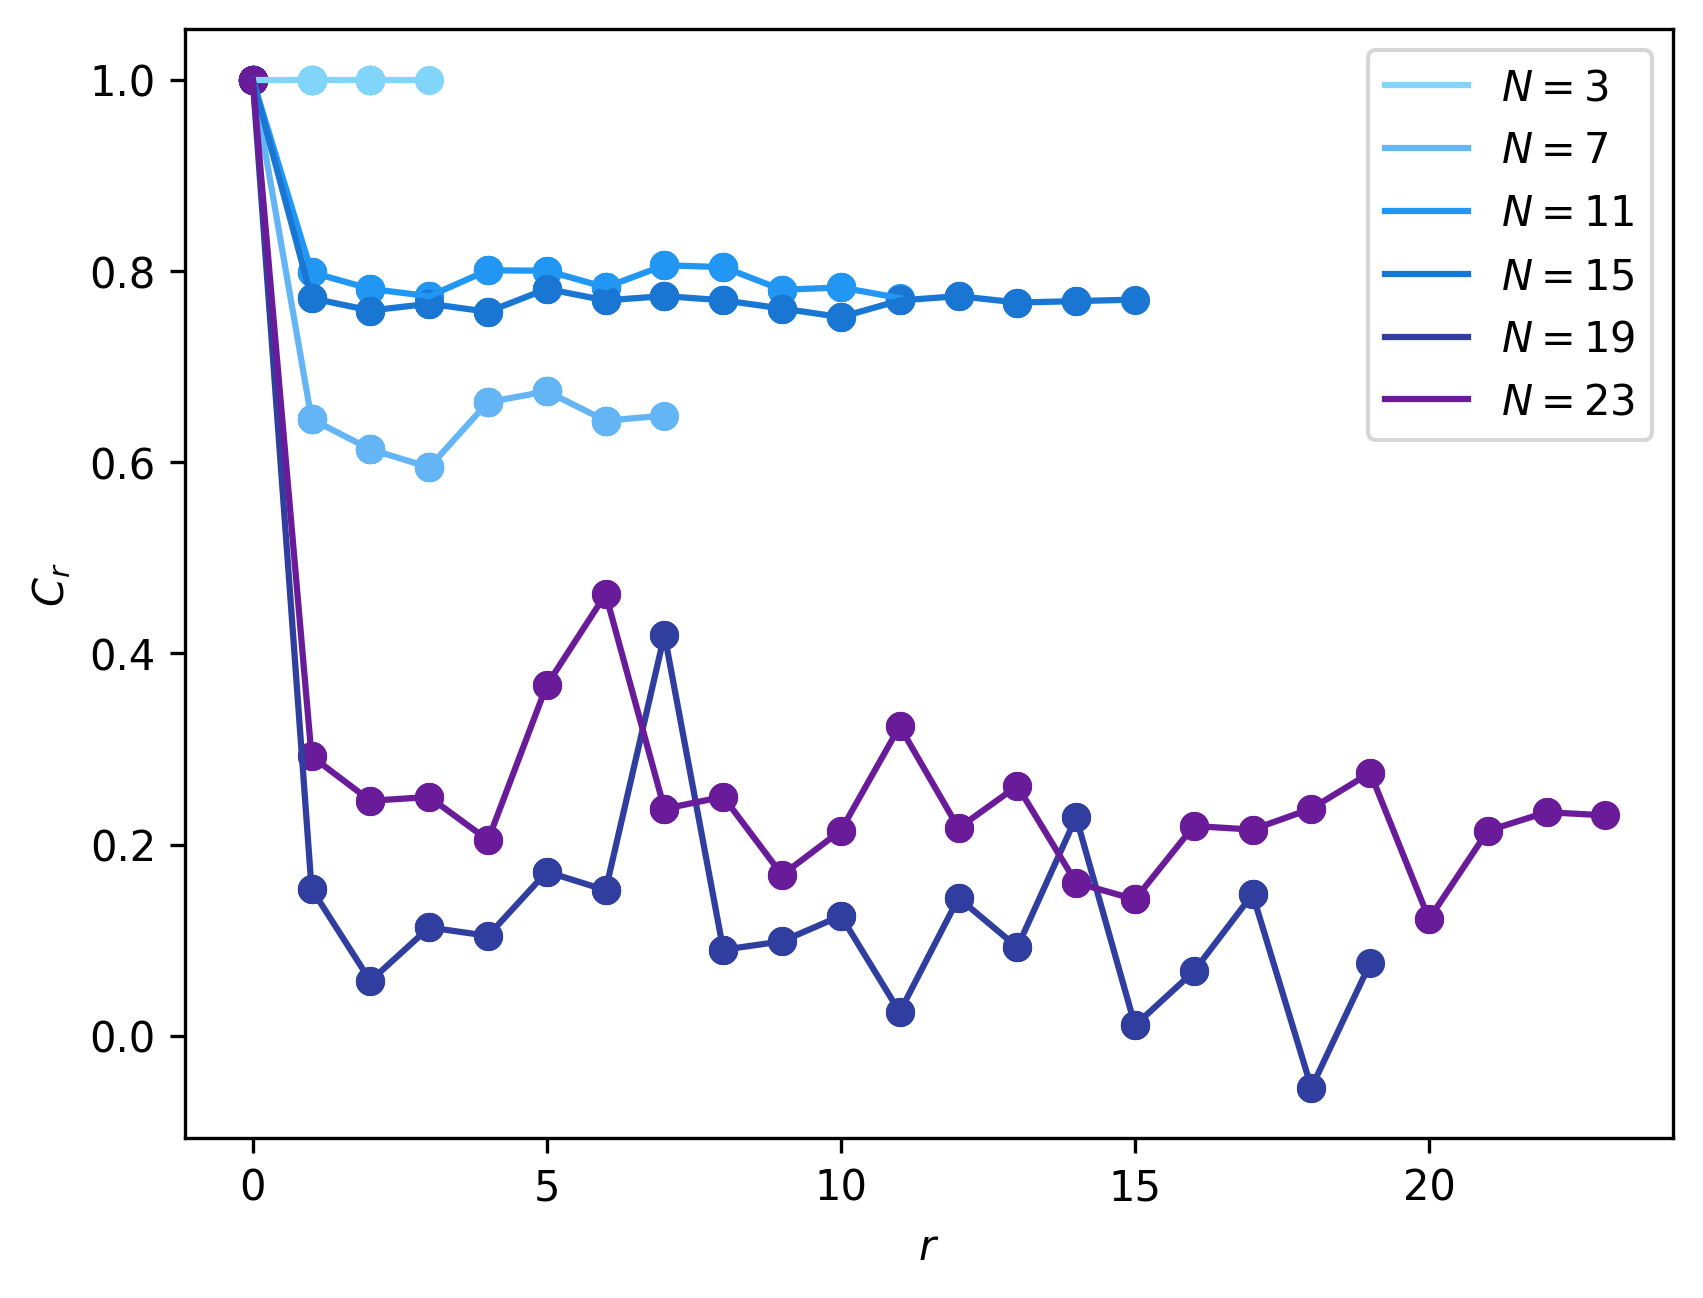
\includegraphics[scale = 0.7]{images/cvr.png}
    \caption{Here we plot the correlation function, $C$ versus $r$}
    \label{fig:c_v_r}
\end{figure}

\section{Autocorrelation time for absolute magnetization}
-
%\begin{figure}[H]
 %   \centering
  %  \includegraphics[scale = ]{}
   % \caption{We have a log-log plot of the autocorrelation time $\tau$ versus the system side size, $N$}
    %\label{fig:c_v_r}
%\end{figure}
\section{Dynamical exponent}
We have,
\begin{equation}
    \tau = N^{z}
\end{equation}
where $\tau$ is the autocorrelation time, $N$ is the number of sites on one side and $z$ is the dynamical exponent. In  the log-log plot of $\tau$ versus $N$, the line traced would follow an equation
\begin{equation}
      \log  \tau = z\log  N
\end{equation}
We can see that the dynamical exponent $z$ appears as the gradient of the plot.
\bibliographystyle{abbrv}
\bibliography{Bibliography.bib}
\end{document}